%
% Apêndices
%
\chapter{Relatórios \textit{p}Nota}
\label{exemplo-pNota}

O \textit{p}Nota tem uma série de relatórios que são utilizados para demonstrar o \textit{status} da avaliação e capacitar a auditoria do processo. Nesse constam os seguintes itens:

\begin{itemize}
\item Lista de Requisição de Amostras
\item Distribuição de \textit{Clusters} de Documentos
\item Distribuição de Treino
\item Distribuição de Características
\item Frequência dos Termos
\item Rubricas por Nota
\item Resultados de Classificação
\item Gráficos de Desempenho
\item Matriz de Confusão
\item Árvore de Decisão
\end{itemize}

Para ilustrar os resultados obtidos com o \textit{p}Nota vamos utilizar um pequeno exemplo. O exemplo é dado pela \textit{Atividade 08b}, extraído do \textit{dataset} do Projeto Feira Literária das Ciências Exatas. O enunciado da questão é dado a seguir:

\begin{quote}
\interlinepenalty=10000
\textit{Em eventos e festas, é comum as pessoas colocarem sal grosso sobre blocos de gelo para manter a temperatura. Por que essa ação mantém o gelo?.}
\end{quote}

A seguir é apresentado o arquivo completo de relatórios e \textit{feedbacks} gerados durante o processo.

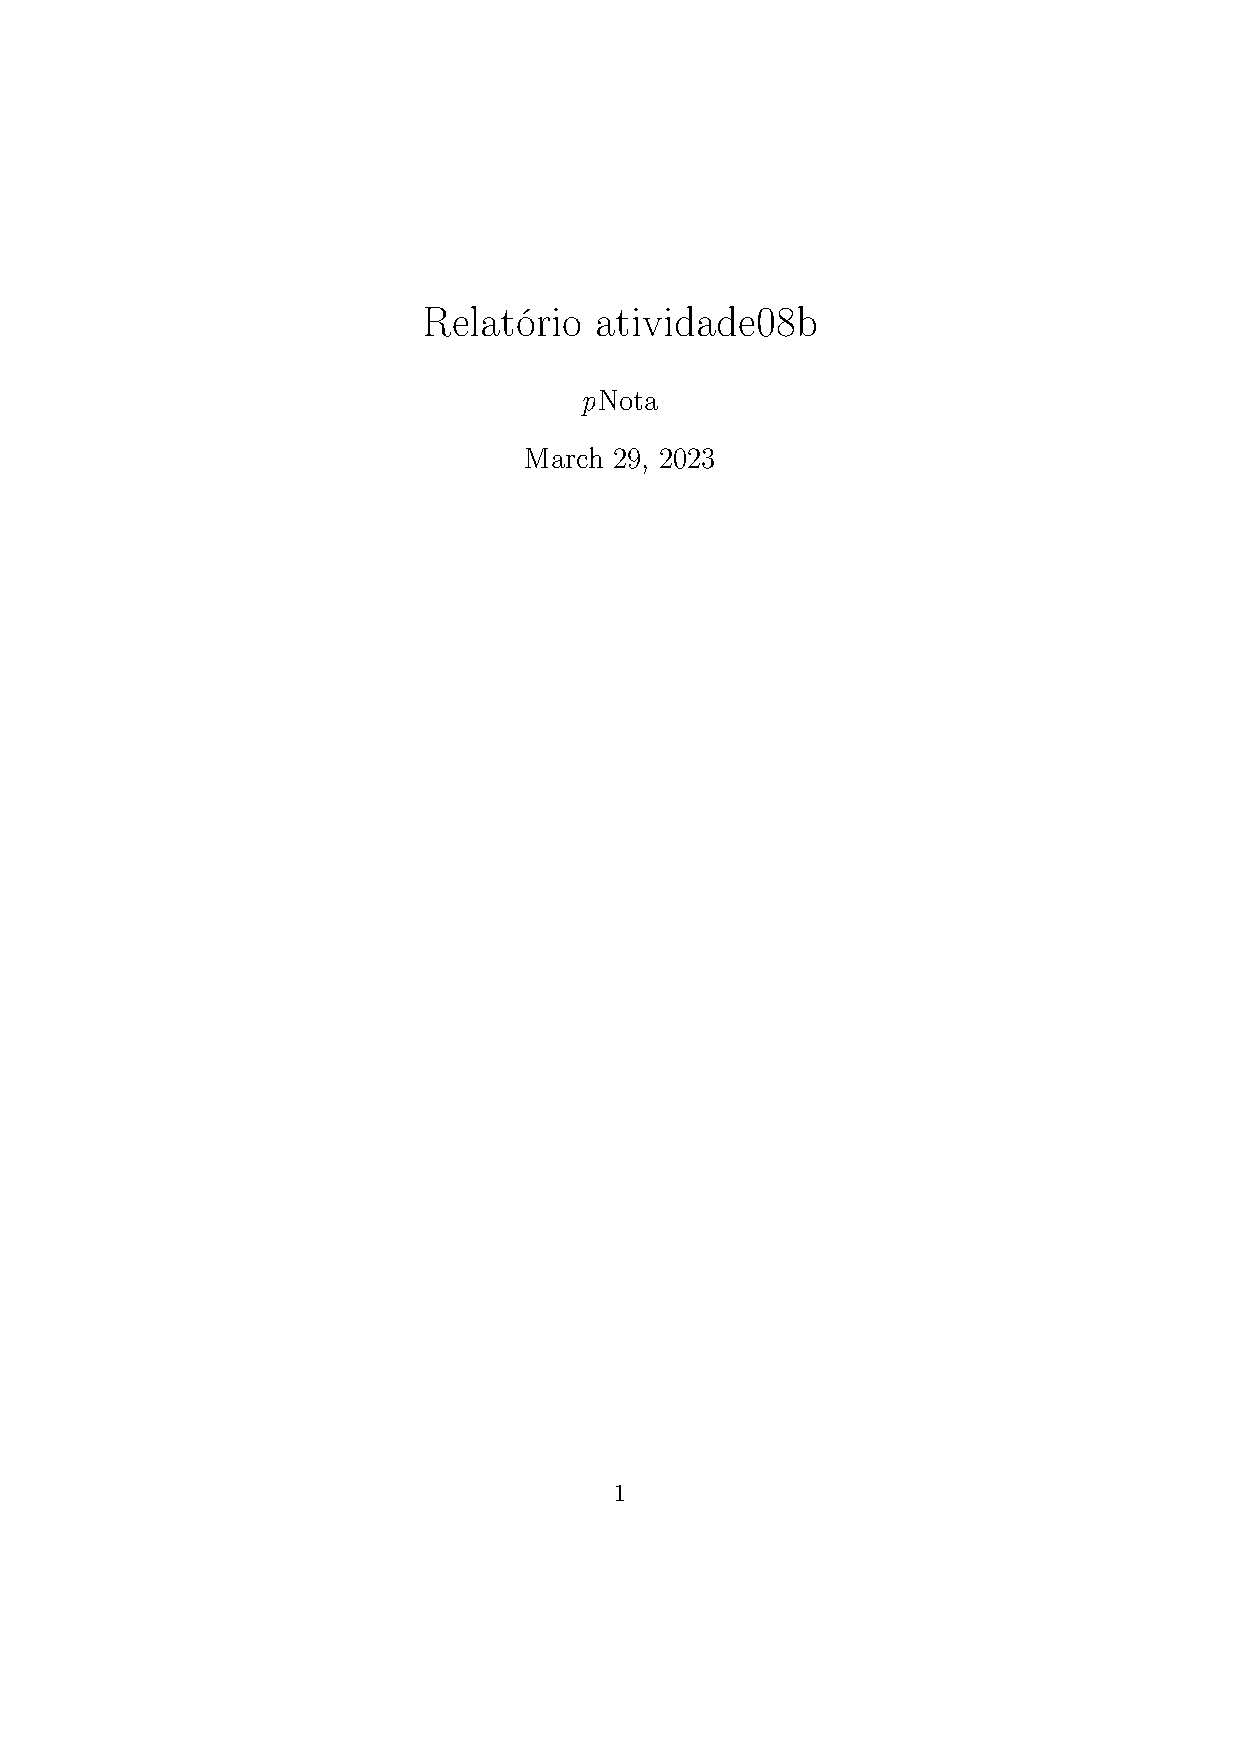
\includepdf[pages={1-}]{relatorio-pNota.pdf}